Numerosi sistemi biologici possono essere modellati con il concetto
astratto di grafo. Studiare la struttura e la topologia di
quest'astrazione non fornisce solo una descrizione dei complessi
comportamenti del sistema in oggetto ma, pu\`o essere di grande
utilit\`a per capire le funzionalit\`a del sistema e le sue dinamiche.

Inoltre attraverso questo processo di astrazione, \`e possibile
studiare quali relazioni possono intercorrere tra il sistema e il
contesto che lo ospita. Lo studio di queste relazioni pu\`o portare a
fare delle stime riguardo la potenzialit\`a del sistema di
``comunicare" con il contesto.

Le idee che abbiamo espresso sono alla base del concetto di
\emph{storia} che avremo modo di studiare meglio nel Capitolo
\ref{chapter:theoretical-background}.  
% A grandi linee una \emph{story}
% \`e un modello di un sistema, con la particolarit\`a di assegnare due
% "ruoli" agli oggetti atomici del sistema. Associeremo uno di questi ad
% un particolare insieme $\mathbb{B}$, i cui elementi (che nel contesto
% biologico sono \emph{metaboliti} o \emph{species}) hanno delle
% caratteristiche di interesse individuate mediante studi
% \emph{empirici}.  Questo lavoro si propone di verificare se sia
% possibile costruire l'insieme $\mathbb{B}$ in modo automatico o, in
% altre parole, se sia possibile attribuire i "ruoli" ai componenti del
% sistema.
\\\\
In questo capitolo, invece, faremo un breve cenno agli oggetti reali
oggetto delle nostre astrazioni, e daremo alcune informazioni sui
metodi e sugli strumenti utilizzati durante lo svolgimento del
progetto.

\section{Metabolic networks, enzimes and pathways}

Prima di definire cosa \`e una \emph{metabolic network} dobbiamo
introdurre i seguenti concetti.

Una \emph{metabolic pathway} \`e una sequenza di reazioni chimiche che
si verificano all'interno di una cellula. Dal punto di vista
matematico, possiamo vedere una metabolic pathway come una sequenza di
funzioni $reaction_{i}$ tali che:
\begin{displaymath}
reaction_{i} : 2^{Molecules} \rightarrow 2^{Molecules}
\end{displaymath}
Ognuna di queste funzioni, avendo in input un insieme di molecole,
esegue delle trasformazioni su queste e produce come output, il
risultato delle trasformazioni svolte sottoforma di insieme di
molecole. Questo output pu\`o essere utilizzato come input per
$reaction_{i+1}$, concatenando quanto si voglia le trasformazioni.
\\\\
Ogni reazione chimica \`e regolata da alcuni \emph{enzymes}. Un
\emph{enzyme} \`e una proteina che gestisce la frequenza e la
velocit\`a di una reazione chimica. Le molecole a cui si applica la
reazione vengono identificate con il termine \emph{substrates} (o
\emph{reactants} usando la terminologia SBML), mentre i prodotti della
reazione vengono indentificati con il termine \emph{products} (anche
la terminologia SBML usa questo identificatore).

Durante l'esecuzione di una reazione chimica, ogni \emph{enzyme}
agisce da \emph{catalyst}, ovvero non viene consumato nella reazione
e, quindi, pu\`o partecipare in pi\`u di una reazione.

L'insieme di \emph{enzymes} "guida" e determina l'insieme di
\emph{pathways} che possono occorrere nella cellula, in quanto una
reazione chimica su un substrato pu\`o avvenire se e solo se lo strato
attivo del substrato complementa quello dell'enzima.

Adesso possiamo definire una \emph{metabolic network} come collezione
di \emph{metabolic pathways}.
\\\\
Nelle prossime sezioni vedremo quali di questi concetti sono necessari
al mio lavoro, cercando di metterli in relazione con le astrazioni
definite dal formato \emph{SBML}.

\section{Code information in SBML format}
Il formato \textbf{SBML} (\textbf{S}ystems \textbf{B}iology
\textbf{M}arkup \textbf{L}anguage) permette di rappresentare
informazioni seguendo uno schema gerarchico, basato su XML.

Questo formato \`e orientato alla descrizione di sistemi in cui
entit\`a biologiche sono oggetto di manipolazioni eseguite da processi
nel corso del tempo, pertanto facilita la codifica di modelli
computazionali di processi biologici, ad esempio \emph{metabolic
  networks, cell-signaling pathways, regulatory networks} e molti
altri. In particolare, le \emph{metabolic network} sono oggetto del
mio elaborato.

\subsection{Model necessary real objects in SBML}
\label{sec:necessaryRealObjectsModeledInSBML}

Nella precedente sezione abbiamo introdotto alcuni concetti che non
sono influenti sul nostro studio, per cui trattiamo solo quelli
inerenti al lavoro che ho sviluppato (molti dei concetti che noi non
usiamo sono comunque modellabili in SBML).

Adesso che abbiamo alcuni concetti reali possiamo iniziare a mapparli
sulle nostre astrazioni, la prima delle quali \`e il mezzo di
comunicazione SBML. Nel seguente \emph{entity diagram} si riportano le
entit\`a di interesse per la nostra trattazione, con le relazioni che
intercorrono tra di esse e gli attributi che possiamo associare a
questi oggetti: \footnote{draw here an entity model that catch the
  fundamental entities.}
\begin{figure}
  \centering
  
  \caption{Fundamental entities}
  \label{fig:FundamentalEntities}
\end{figure}
Le unit\`a atomiche definibili con SBML sono le \emph{species}. Una
\emph{species} rappresenta il concetto di molecola (appartenente ad
almeno un \emph{substrate}).  Un oggetto di tipo \emph{species} ha
molti attributi ma, ai nostri fini, tre sono quelli necessari:
\begin{itemize}
\item \emph{identifier}, che permette di assegnare una etichetta univoca
alla specie all'interno di tutto il modello SBML
\item \emph{name}, che permette di codificare delle informazioni di
  pi\`u alto livello rispetto all'\emph{identifier}
\item \emph{compartment}, che permette di assegnare ad una specie il
compartimento della cellula dove risiede (in tutti gli esempi che
abbiamo avuto modo di testare il compartimento \`e sempre il
citoplasma).
\end{itemize}

Un altro concetto fondamentale \`e quello di \emph{chemical reaction},
codificato in SBML con:
\begin{itemize}
\item \emph{reactants}, insieme di \emph{species}, che modellano il
  \emph{substrate} della reazione.
\item \emph{products}, insieme di \emph{species}, che modellano i
  prodotti della reazione.
\end{itemize}
Inoltre \`e necessario modellare il concetto di reazione
reversibile, il quale viene catturato in SBML dal flag
\emph{reversible}.
\\\\
Questo \`e quello che ci serve per iniziare ad analizzare il modello
SBML: ricercheremo l'insieme di reazioni descritte e, per ogni
reazione, analizzeremo l'insieme dei \emph{reactants} e dei
\emph{products} per costruire un nostro modello sul quale implementare
i nostri algoritmi.
\\\\
Nella prossima sezione descriveremo le regole che abbiamo utilizzato
per costruire, dato in input un modello SBML, il nostro modello
dati.

\subsection{SBML model $\rightarrow$ Our model}

Abbiamo la necessit\`a di modellare i concetti espressi in formato
SBML con un nostro modello in quanto ci permette di ridurre la
complessit\`a delle informazioni e ci permette di applicare in modo
semplice molti algoritmi presi dalla teoria dei grafi.

Senza questo nostro modello la trattazione del problema sarabbe molto
complicata e non ci permetterebbe di arrivare a dei
risultati\footnote{Qui potrebbe essere il caso di inserire
  l'osservazione che fece Andrea sugli ipergrafi, che renderebbero il
  problema NP-completo. Mi ricordo bene?}.
\\\\
Il nostro modello \`e essenzialmente un grafo orientato, la cui
caratteristica \`e quella di catturare l'idea dei nodi \emph{black} e
nodi \emph{white} (vedi \cite{tellingStories}), essenziali per
l'astrazione di \emph{story}.

Per costruire questo modello usiamo questo insieme di regole:
\begin{itemize}
\item due specie sono uguali se hanno uguale identificatore ed uguale
  compartimento. Questa regola \`e necessaria per evitare una
  esplosione di nodi del nostro modello in quanto, date due reazioni
  $r$ e $r'$, se $a \in reactants(r) \wedge a' \in reactants(r')$ con
  $a = a' \wedge r \not = r'$, si costruirebbero due nodi distinti
  rispettivamente per $a, a'$, non si avrebbero informazioni
  significative in quanto il grafo degenerebbe ad un insieme di
  sottografi isolati, ognuno rappresentante una reazione. Quindi una
  specie non \`e identificata dalle reazioni in cui appare.
\item data una reazione non-reversibile $r$ tale che:
  \begin{displaymath}
    \begin{split} 
      reactants(r) &= \{ r_{1}, \ldots, r_{n} \} \\
      products(r) &= \{ p_{1}, \ldots, p_{m} \}
    \end{split}
  \end{displaymath}
  allora il nostro modello sar\`a uguale al grafo che codifica la
  relazione $reactants(r) \times products(r)$. Ad esempio, con
  $reactants(r) = \{ a, b, c, d \}$ e $products(r) = \{a, e, f\}$
  otteniamo:

\begin{figure}[!htb]
\centering
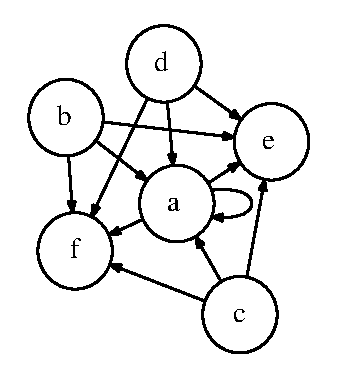
\includegraphics{images/non-reversible-reaction-example.dot.eps}
\end{figure}
supponendo che la specie $a$ appartenente ad entrambi gli
insiemi sia la stessa (ovvero se $\exists a': a = a' \rightarrow id(a) =
id(a') \wedge compart(a) = compart(a')$).

\item data una reazione reversibile $r$ tale che:
  \begin{displaymath}
    \begin{split} 
      reactants(r) &= \{ r_{1}, \ldots, r_{n} \} \\
      products(r) &= \{ p_{1}, \ldots, p_{m} \}
    \end{split}
  \end{displaymath}
  allora il nostro modello sar\`a uguale al grafo che codifica la
  relazione $(reactants(r) \times products(r)) \cup (products(r)
  \times reactants(r))$. Ad esempio, con $reactants(r) = \{ a, b, c, d
  \}$ e $products(r) = \{a, e, f\}$ otteniamo:

\begin{center}
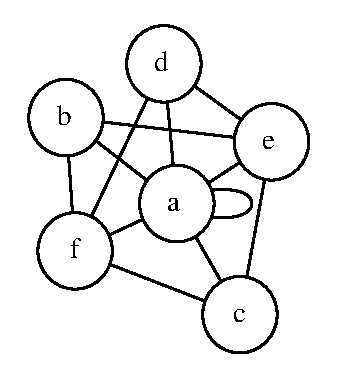
\includegraphics{images/reversible-reaction-example.dot.eps}
\end{center}
supponendo che la specie $a$ appartenente ad entrambi gli
insiemi sia la stessa (ovvero se $\exists a': a = a' \rightarrow id(a) =
id(a') \wedge compart(a) = compart(a')$).

\end{itemize}

Nella prossima sezione descriveremo alcuni dettagli e caratteristiche
di modelli SBML che non sono esplicitamente documentate sul sito
ufficiale (vedi \cite{sbmlOfficialDocumentation}), ma che abbiamo
capito e dedotto utilizzando il concetto di \emph{learning test} (vedi
\cite[p. 136]{beck2003}) implementato con \emph{JUnit}.

\subsection{Learning SBML tips by tests}

Scrivendo alcuni \emph{learning tests} abbiamo dedotto le seguenti
propriet\`a sui modelli SBML. I seguenti test sono stati esercitati su
una batteria di modelli biologici reali, tutti con esito positivo:
\begin{itemize}
\item sia $r$ una reazione e siano $reactants(r), products(r)$ gli
  insiemi di \emph{reactants} e \emph{products}
  rispettivamente. Questi due insiemi catturano il concetto di insieme
  matematico, ovvero non contengono oggetti duplicati.
\item $\exists r,t \in Reactions: products(t) = reactants(r)$. Questa
  propriet\`a permette di avere continuit\`a tra reazioni, ovvero un
  insiemi di \emph{products} di una reazione $t$ pu\`o essere
  l'insieme di \emph{reactants} di una reazione $r$. Questa
  propriet\`a permette di costruire delle \emph{metabolic pathways}
  composte da quante reazioni si voglia.
\item ogni species deve essere contenuta in un compartment.
\item l'identificatore discrimina le species, ovvero se tentiamo di
  aggiungere al modello due species con lo stesso identificatore, ma
  contenute in compartimenti diversi, allora nel modello viene
  inserita una delle due ma non entrambe, scegliendo in ordine
  cronologico di inserimento
\end{itemize}

\section{About this work}
In questa sezione riportiamo delle informazioni riguardo alla libreria
java che abbiamo sviluppato, daremo una sinopsi della struttura di
questo documento e riporteremo alcuni dettagli tecnici relativi agli
strumenti utilizzati per la realizzazione dell'intero lavoro.

\subsection{The java library}
Il mio lavoro ha prodotto una libreria java nella quale vengono
implementati i concetti esposti nel capitolo
\ref{chapter:theoretical-background} e si prefigge di essere
utilizzata non come un programma a se stante, bensi \`e molto pi\`u
orientata ad un utilizzo programmatico. Per questo motivo abbiamo
ritenuto opportuno riportare nella sezione
\ref{section:packages-descriptions} una descrizione di ogni
\emph{package} in modo da favorirne la comprensione e
l'utilizzo. Nella libreria \`e presente anche una maschera realizzata
utilizzando il framework \emph{SWING} per la renderizzazione di un
particolare set di output relativi alla composizione delle strongly
connected components: questo \`e l'unico oggetto che non \`e possibile
utilizzare programmaticamente.

\subsection{Sinopsi}
In questa sezione elenchiamo i capitoli in cui questo documento \`e
suddiviso e, per ognuno di assi, daremo una breve descrizione del
contenuto.

Il capitolo \ref{chapter:introduction} contiene una introduzione al
lavoro svolto. Vengono introdotti i concetti chiave del problema in
questione, il formato di codifica delle informazioni \emph{SBML}, come
catturare le informazioni in questo formato ed alcuni dettagli tecnici
relativi alla realizzazione del progetto.

Il capitolo \ref{chapter:theoretical-background} modella da un punto
di vista teorico i concetti e gli algoritmi alla base delle
implementazioni. Verr\`a precisato il concetto di \emph{story} e il
significato dell'insieme $\mathbb{B}$, cosa significa eseguire una
visita di un grafo, approfondiremo la strategia \emph{Depth First} e
si studieranno tre algoritmi per la ricerca di \emph{strongly
  connected components}.

Il capitolo \ref{chapter:study} formalizza gli obiettivi che vogliamo
raggiungere con lo sviluppo della libreria java. Vengono proposti gli
\emph{use-case} che abbiamo implementato e, per ognuno di essi,
vengono riportati degli esempi del "prodotto finito" in modo da dare
un'idea se non si \`e avuto modo di utilizzare la libreria. Inoltre si
analizza l'architettura che caratterizza l'intera implementazione.

Il capitolo \ref{chapter:implementation} affronta tutte le questioni
inerenti alla fase di implementazione. Si affronta la metodologia di
sviluppo utilizzata, alcuni paradigmi e idiomi usati ripetutamente
durante la fase di codifica ed una breve descrizione dei
\emph{package} che compongono il progetto.

Il capitolo \ref{chapter:conclusions} termina il lavoro esponendo i
risultati ottenuti ed elencando una lista di sviluppi futuri del
progetto.

\subsection{Used tools}
Per lo sviluppo di questo progetto sono stati utilizzati i seguenti
strumenti:
\begin{itemize}
\item per la stesura di questo documento \`e stato usato il motore di
  formattazione \TeX, utilizzando \emph{Emacs} come editor dei file
  sorgenti, installando la \emph{mojor mode AucTex}
\item l'implementazione della libreria java \`e stata sviluppata
  completamente con \emph{Eclipse} versione \emph{Indigo}
\item i sorgenti, sia dell'elaborato testuale sia
  dell'implementazione, sono stati versionati utilizzando il sistema
  \emph{Git}. Abbiamo utilizzato \emph{Github} come provider del
  servizio. I sorgenti di questo documento possono essere scaricati
  dall'URL:\\
  % \href{https://github.com/massimo-nocentini/my-undergraduate-thesis}{
  %   https://github.com/massimo-nocentini/my-undergraduate-thesis}\\
  % mentre i sorgenti dell'implementazione java dall'URL:\\
  % \href{https://github.com/massimo-nocentini/my-undergraduatethesis-java}{
  %   https://github.com/massimo-nocentini/my-undergraduatethesis-java}
\end{itemize}

\subsection{Feedback}
Per riportare consigli, correzioni o domande \`e possibile inviare una
mail all'indirizzo \\
\href{massimo.nocentini@gmail.com}{massimo.nocentini@gmail.com}
